% !TEX root = mythesis.tex

%==============================================================================
\chapter{Experimental equipment}
\label{sec:LHCATLAS}
%==============================================================================

\section{The Large Hadron Collider}
The Large Hadron Collider is a two-ring proton-proton collider situated near Geneva across the Swiss-French border. It is built in the 26.7 km long tunnel 
that previously housed the Large Electron-Positron (LEP) collider. The two proton beams are accelerated in opposite directions and brought into collision at 
four points where the four detectors are located. The LHC has two tranfer tunnels of 2.5 km each that connects to the CERN accelerator complex as shown in 
\cref{fig:acc_complex}. Each system in this complex contributes to the acceleration of protons. Negative Hydrogen ions are are accelerated in LINAC4 which 
is the first system in the CERN accelerator complex. Electrons are stripped off from hydrogen ions during injection from LINAC4 to Proton Synchrotron Booster (PBS) 
which further accelerates the protons. Eventually the accelerated protons are fed into the Super Proton Synchrotron (SPS). At this point proton energy is 450 GeV 
when they are finally injected into two opposing beams of the LHC. Here each beam attains a path-breaking energy of 6.5 TeV. 

\begin{figure}[htbp]
    \centering
    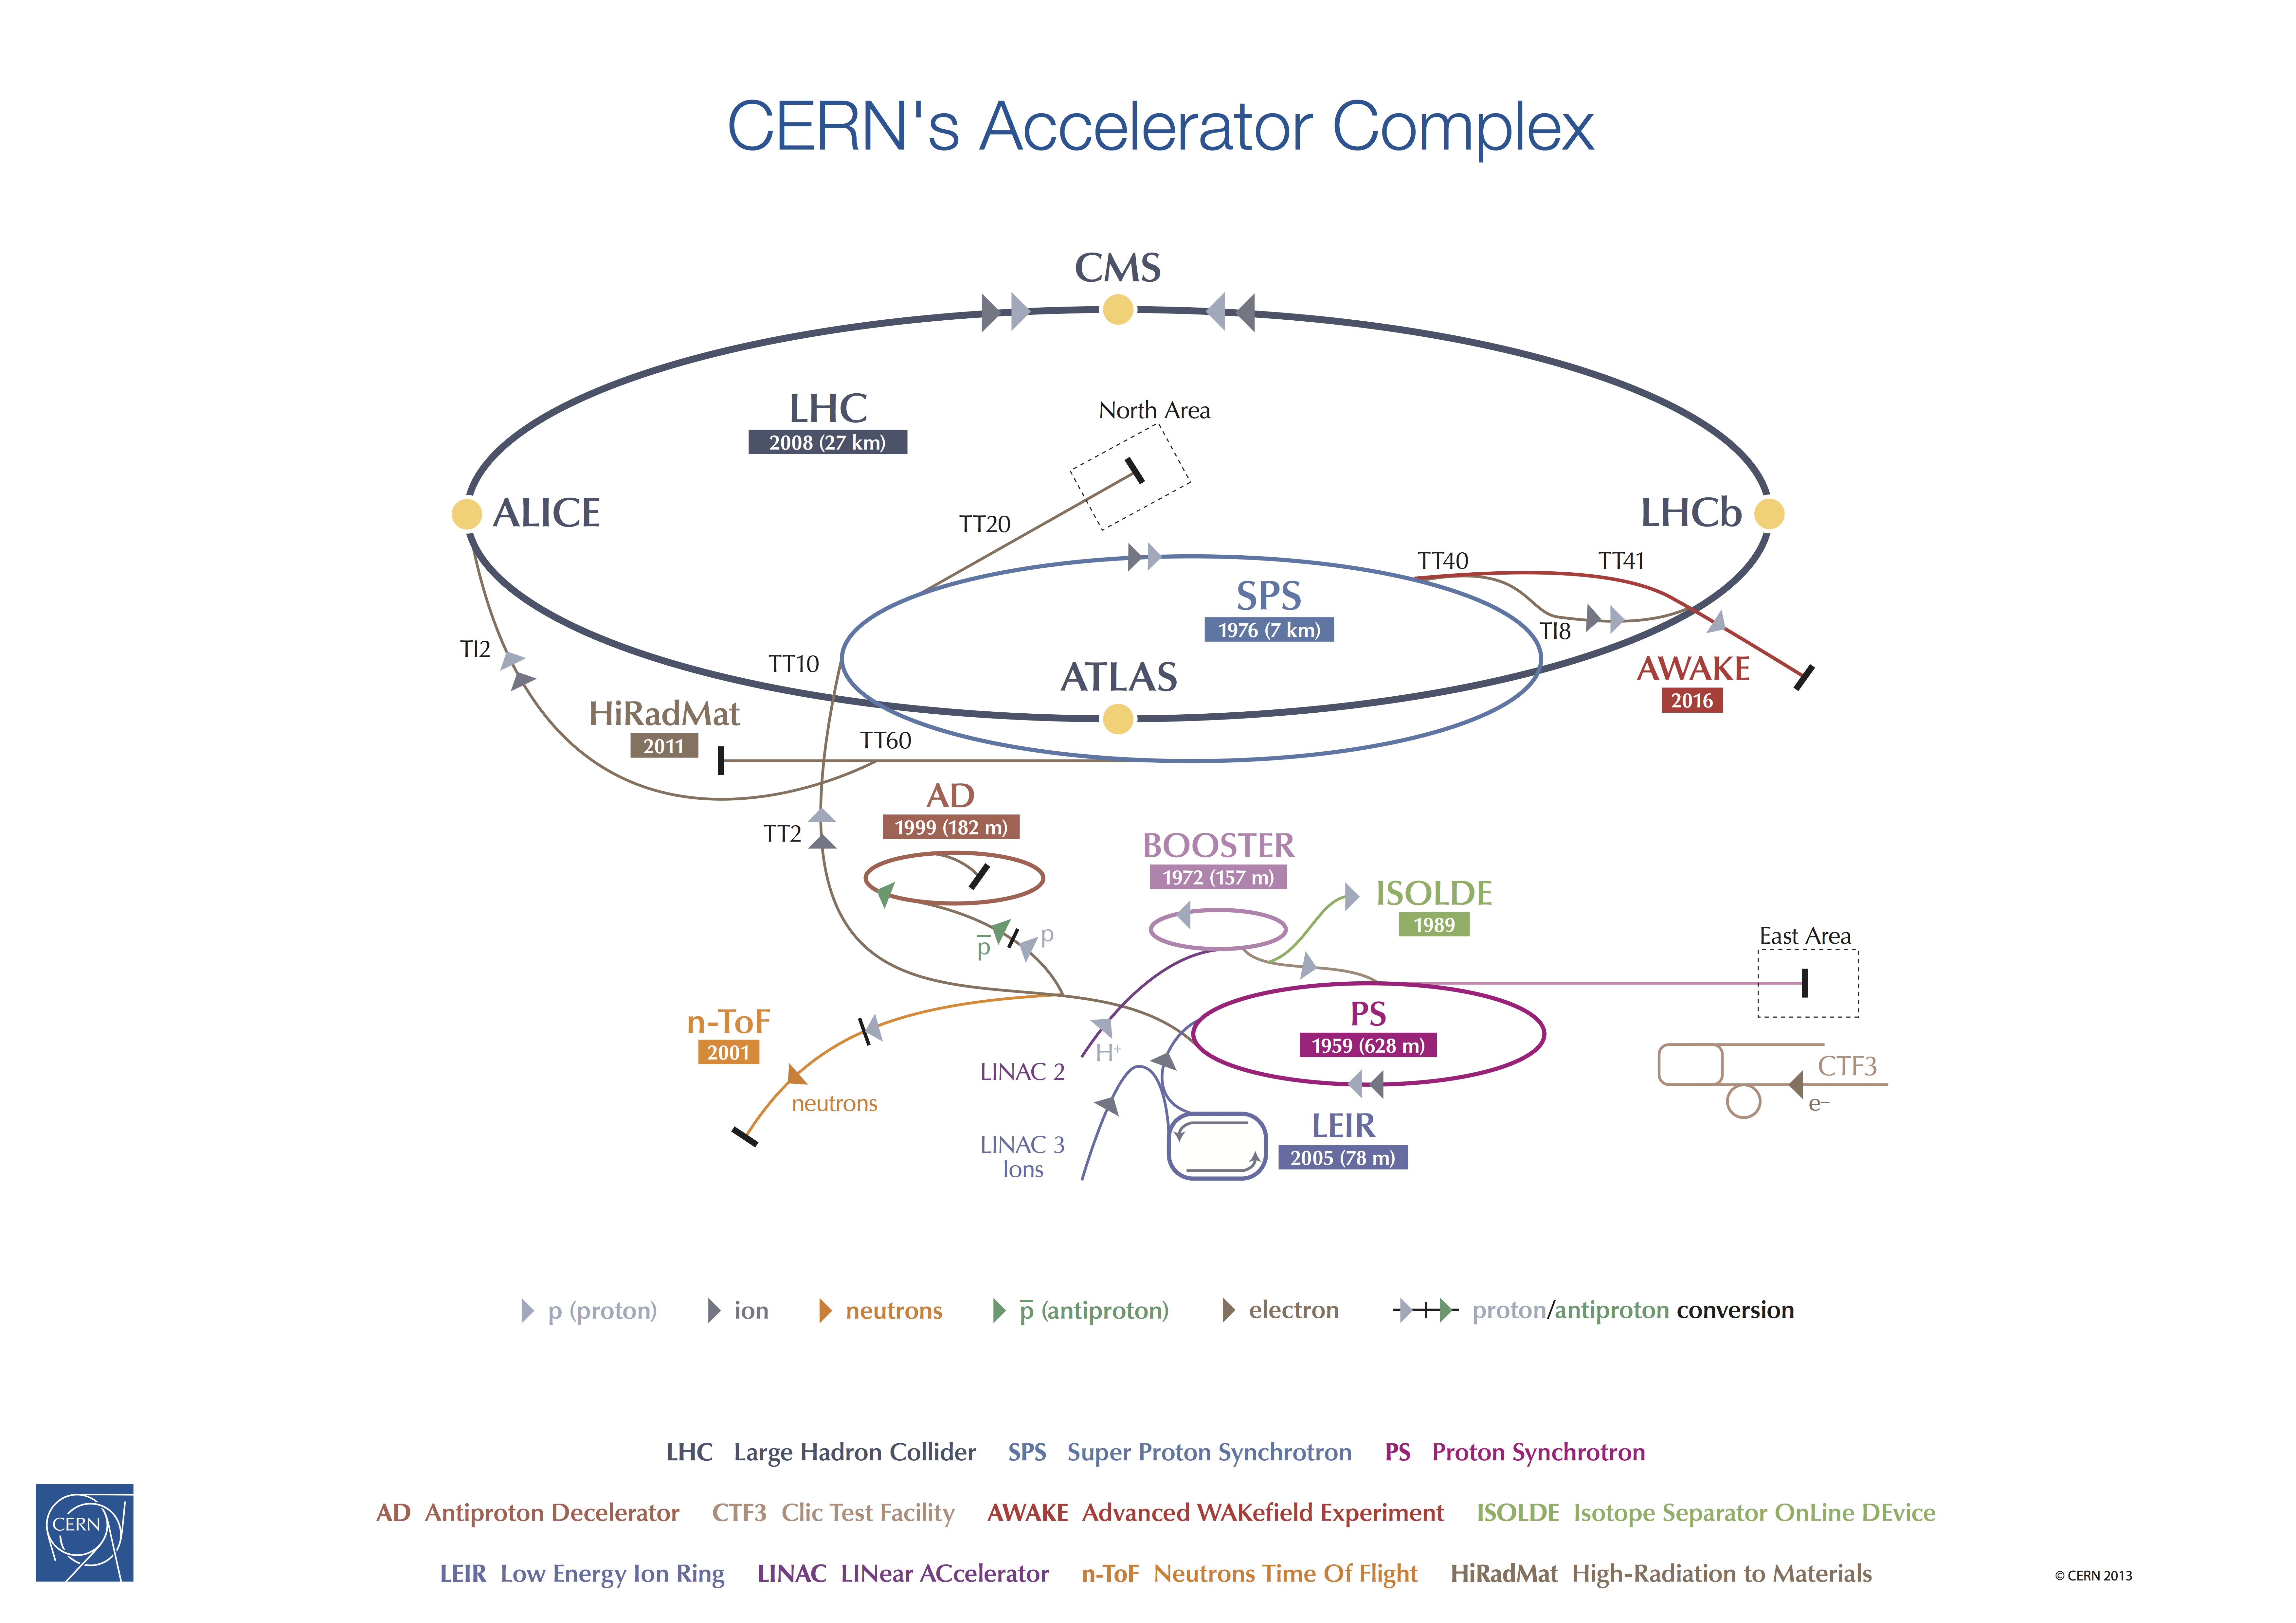
\includegraphics[width=\figwidth]{Poster-2013-377.jpg}
    \caption[Sketch of the CERN accelerator complex]{Sketch of the LHC ring along with the machines in the CERN accelerator complex\cite{Haffner:1621894}.}%
    \label{fig:acc_complex}
\end{figure}


The proton beams need to be directed along the circular structure of the LHC. To achieve the destined center of mass energy, given the circumference and charge
of proton, around 8 T magnetic field is required. This is outside the limit of conventional magnets which is why superconducting magnets are used. Due to the limited
area in the LHC tunnel, a single magnet system is shared by both the beam pipes. The superconducting coils are immersed in a superfluid Helium bath
that is cooled down to a certain low temperature to achieve superconductivity. One of the obstacles here is the synchrotron radiation. The accelerating protons 
radiate photons when they are accelerated and this radiation can adversely impact the temperature inside the magnet system. To fix this problem there are beam 
screens placed between the beam pipe and the magnet system that reflects or absorbs these photons and hence protects the superconductivity. 

Luminosity ($L$) defines the number of a certain type of reaction in collisions. The number of reactions can be determined as $L\sigma$ where $\sigma$ is the 
probability of a certain reaction and it is called cross-section. For a particle collider, beam energy and luminosity are two important figures of merit. High energy
allows production of new heavy particles and high luminosity allows more flux of particles contributing to high number of collisions. 